\documentclass{IEEEtaes}

\usepackage[T1]{fontenc}
% Use the TAES submission dimensions with the journal's production class.
\renewcommand{\CLASSINFOpaperwidth}{8.5in}
\renewcommand{\CLASSINFOpaperheight}{11in}
\setlength{\hoffset}{0pt}
\setlength{\voffset}{0pt}
\usepackage[letterpaper,top=1in,bottom=1in,left=0.7in,right=0.7in,columnsep=0.2in]{geometry}
\usepackage{amsmath,amssymb}
\usepackage{graphicx}
\usepackage{booktabs,array}
\usepackage{cite}

\newcommand{\pos}[1]{\left[#1\right]_+}
\newcommand{\dd}{\mathrm{d}}

% Keep only correspondence and page numbers from the production footer.
\makeatletter
\let\taesproductionmaketitle\maketitle
\renewcommand{\maketitle}{%
  \let\taesproductionfootnotetext\footnotetext
  \renewcommand{\footnotetext}[1]{\taesproductionfootnotetext{\noindent\@corresp}}%
  \taesproductionmaketitle
  \let\footnotetext\taesproductionfootnotetext
}
\def\ps@taesreview{%
  \let\@oddhead\@empty
  \let\@evenhead\@empty
  \def\@oddfoot{\hbox to \textwidth{\footnotesize Orbital Engineering Lab / Original Research\hfil\thepage}}%
  \let\@evenfoot\@oddfoot
}
\makeatother
\hypersetup{hidelinks,pdftitle={Cooperative Spacecraft Docking with Time-Limited Readiness Guarantees},
  pdfauthor={Adam Cohen}}

\begin{document}
\pagestyle{taesreview}

\title{Cooperative Spacecraft Docking with Time-Limited Readiness Guarantees}
\author{Adam Cohen}
\affil{Orbital Engineering Lab}
\corresp{Corresponding author: Adam Cohen (\href{mailto:adamhcohen8@gmail.com}{adamhcohen8@gmail.com}).}
\markboth{IEEE TRANSACTIONS ON AEROSPACE AND ELECTRONIC SYSTEMS}
{COOPERATIVE SPACECRAFT DOCKING}
\maketitle
\thispagestyle{taesreview}

\begin{abstract}
A chaser approaching a docking port must decide whether the receiver will stay ready through contact. We bound the time left on a receiver commitment using two clocks with bounded drift and derive the axial acceleration commands that guarantee first contact within a specified speed band. Two encounters with identical chaser observations illustrate the value of measuring receiver turnaround. One admits a safe command. In the other, even maximum acceleration falls 10.34 mm short in an allowed realization. In 21 matched Orbital Engineering Lab (OEL) profiles, a fixed delay bound yielded 15 modeled captures. Adding chaser elapsed time with no positive processing minimum yielded 17, and adding receiver turnaround yielded 20. A chaser given the simulator's 62.5 ms processing minimum matched the turnaround policy's capture decisions across all 57 profiles. In a prospective geometry test, OEL reproduced all five predicted higher-tilt crossings of the port-center timing bound. Accounting for the leading edge enclosed all ten tested contacts. The guarantee assumes bounded approach dynamics and an honored receiver commitment.
\end{abstract}

\begin{IEEEkeywords}
Autonomous spacecraft, clock uncertainty, rendezvous and docking, runtime assurance.
\end{IEEEkeywords}

\section{Introduction}

Two cooperative spacecraft may exchange readiness indications before final approach. A READY message certifies a past state. If the receiver can withdraw readiness while the chaser is still acting on the message, the chaser may cross its stopping boundary before learning of the withdrawal. A shorter freshness timeout can prevent this behavior at the expense of early holds or retreats. Inter-spacecraft refueling interfaces already specify a readiness exchange and reconfirmation \cite{ior}, and the HTV-X safety study analyzes timing disagreements in docking and abort sequencing \cite{htvx}. The question addressed here is what a readiness exchange must establish before a vehicle may commit to contact.

Breeden and Panagou show finite-time docking under bounded disturbances using robust control barrier functions and a nonmaneuvering target \cite{breeden}. Bresch-Pietri and Del Vecchio derive distributed collision-avoidance controls for bounded time-varying communication delay \cite{bresch}. Dunlap et al. compare runtime assurance filters for velocity-constrained three-dimensional docking \cite{dunlap}. In ground traffic, Dresner and Stone reserve space and time for vehicles traversing an intersection \cite{dresner}. Here the reserved resource is a partner's continued readiness. The clocks may have unrelated epochs, and a delayed command must place the entire reachable first-contact window inside the remaining grant. A further interval covers the handoff.

The timing rule draws on distributed leases \cite{gray,nerio} and the subtraction of remote turnaround in network delay measurement \cite{ntp}. Nerio's bounded-drift protocol anchors the requester's guarantee to its initiation time. Here the receiver starts the commitment after arming, and its measured turnaround reduces the worst-case age of that commitment at the decision. The technical contribution is the composition of that bound with delayed control and the geometry of first contact. This composition yields an explicit command interval and identifies when better timing information can change the decision.

This paper derives a tight readiness-time bound for the stated timing information, a contact certificate with an explicit interval of admissible commands, and a correction for contact at the edge of a tilted port. The evaluation holds the guidance law fixed across timing policies, gives the fixed-delay baselines a chance to recover by renewing their grants, and tests both timing and geometry near their predicted boundaries. The scope is first contact and a prescribed handoff interval in a cooperative terminal approach. Physical latch reliability, loads and hard mate are outside the tested envelope.

\section{Time-Limited Receiver Readiness}
\label{sec:contract}

\begin{figure*}[!t]
\centering
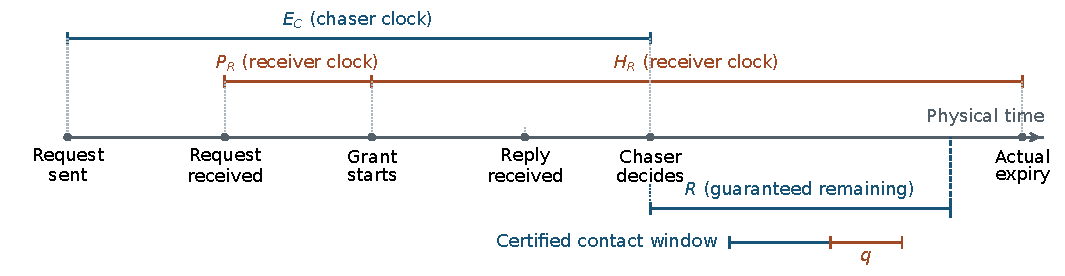
\includegraphics[width=\textwidth]{readiness-timeline.pdf}
\caption{Illustrative readiness exchange on a common physical-time axis. The chaser measures $E_C$ on its clock. The receiver measures $P_R$ and promises $H_R$ on its clock. At the decision, the computed remaining interval $R$ must cover the latest certified contact and the subsequent handoff reserve $q$. Actual expiry is visible to the scorer.}
\label{fig:timeline}
\end{figure*}

\subsection{Immediate Revocation}

Assume that the receiver may withdraw readiness while its precontact motion stays the same, and that delivery of the withdrawal may occur after first contact. Consider two executions with identical chaser observations through contact. The receiver remains ready in one execution and withdraws in the other. Because the chaser has the same information and the same physical inputs in both, a chaser that makes contact in the first execution also makes contact in the second. Under these conditions, a guarantee against unarmed contact requires additional information or a physical constraint on withdrawal. Improved relative navigation alone cannot distinguish the two executions.

\subsection{Residual-Time Bound}

The chaser timestamps a request on its own monotone clock. After arming the interface and satisfying its motion bounds, the receiver starts a reservation. It returns the request identity, its promised interval $H_R$ in receiver-clock seconds, and its measured turnaround $P_R$ from receipt of the request to reservation start. Duplicates retain the original identity and expiry. An old reply cannot extend a different reservation.

Let the instantaneous clock rate of vehicle $i$ be in $[1-\rho_i,1+\rho_i]$ relative to physical time, with $0\leq\rho_i<1$. The clock epochs may be arbitrary. At the chaser's decision, $E_C$ is the local elapsed time since the request. The corresponding physical interval is $F+P+B$, where $F$ is outbound delay, $P$ is receiver turnaround, and $B$ is the reservation's age at the decision. The last term includes reply transmission, queueing and any wait at the chaser.

Fig.~\ref{fig:timeline} shows the measured intervals and the deadline used by the contact certificate.

\emph{Proposition 1:} From these observations and $F\geq0$, the remaining readiness in physical seconds is at least
\begin{equation}
R = \frac{H_R}{1+\rho_R}
 - \max\left(0,\frac{E_C}{1-\rho_C}
              -\frac{P_R}{1+\rho_R}\right).
\label{eq:remaining}
\end{equation}

\emph{Proof:} The physical elapsed time is at most $E_C/(1-\rho_C)$. The receiver spent at least $P_R/(1+\rho_R)$ before the reservation started. Subtracting this lower bound and using $F\geq0$ gives the upper bound on $B$ in \eqref{eq:remaining}. The receiver's promise lasts at least $H_R/(1+\rho_R)$ in physical time. For consistent observations, the bound is attained in the information model by choosing the slowest chaser clock, the fastest receiver clock and $F=0$. Clocks may therefore have arbitrary epochs. Timestamp quantization is handled by rounding $E_C$ up and $P_R$ down. \hfill$\square$

If an independently established upper bound $\bar B$ covers reservation age at the decision, the chaser can use the smaller of that bound and the age term in \eqref{eq:remaining}. Equivalently, it takes the larger of the two valid remaining-time bounds. Without a turnaround measurement the chaser may use a documented physical processing minimum $P_{\min}$ in place of $P_R/(1+\rho_R)$ in the age bound. If the interface specifies no positive minimum, it uses zero. The elapsed-time argument does not require a delivery deadline for safety. A lost or late reply can prevent progress, and a successfully admitted approach can finish during subsequent silence if the receiver honors its existing promise. Failure of the mechanism, receiver motion outside the contract, or an early withdrawal after a valid grant requires a separate contingency response.

\subsection{Receiver Contract}

The receiver transitions from available to reserved only after it has armed the capture mechanism and established that its attitude and motion can stay within the declared envelope for the grant duration. Admission reserves both the mechanism state and the authority to inhibit incompatible maneuvers. The grant ledger binds the request and session identity to a fixed expiry on a monotonic receiver clock. Repeated replies return the same grant. A distinct renewal adds an interval, and the receiver retains the obligation throughout the union of unexpired intervals, including when a reply is lost. When the final grant expires, reserve release is allowed under the encounter's postcontact or retreat rules.

A routine reset or incompatible abort request must be deferred while an obligation is active, or handled by a lower-level interlock that preserves arming, the motion envelope and expiry across the transition. A practical reset-tolerant implementation would require a retained clock and ledger plus authority to maintain the mechanism and motion bounds. A fault that defeats those elements invalidates the premise of the guarantee. The simulations model the retained obligation and communication loss. The study receiver stores the original duration, turnaround and expiry for each identity within the session. Its chaser ignores replies generated by duplicate requests because the fixed delay guarantee applies to the original transmission. Supplement Sec.~S4 tests the implementation against a separate specification.

\section{Contact and Retreat Certificates}
\label{sec:guidance}

\subsection{Stopping Reserve Before Commitment}

Let $g$ be axial clearance and $v$ positive closing speed. Let $d$ bound adverse relative acceleration, $b>d$ be commanded braking acceleration, and $\ell$ be the longest delay until braking takes effect. For an upper closing speed $\bar v$, the closure before the first stop is bounded by
\begin{equation}
D(\bar v,\ell)=
  \bar v\ell+\frac{d\ell^2}{2}
  +\frac{(\bar v+d\ell)^2}{2(b-d)}.
\label{eq:stop}
\end{equation}
The first two terms bound travel before braking. The last term uses the minimum net deceleration and the largest possible speed at brake onset. The chaser admits a waiting action only if its lower clearance is at least $r+D$ for the control period plus the maximum actuation lag, with $r$ a required separation reserve. If that test cannot be renewed at the next decision, the retained margin allows braking. The initial state must admit immediate braking. The bound applies through the first stop. Subsequent departure and conjunction safety have separate requirements.

\subsection{Commitment to First Contact}

At the commitment decision, let initial clearance and speed be in boxes $g\in[g_-,g_+]$ and $v\in[v_-,v_+]$. The chaser selects an inward acceleration $u\in[0,u_{\max}]$ that is constant after an uncertain actuation lag $\ell\in[\ell_-,\ell_+]$. The precontact axial dynamics are
\begin{equation}
\dot g=-v,\qquad
\dot v=u\,\mathbf{1}_{t\geq \ell}+w(t),\qquad
|w(t)|\leq d.
\label{eq:model}
\end{equation}
The disturbance covers the receiver's allowed axial acceleration and differential gravity in the final-approach envelope. If $q$ denotes a reserved handoff interval, the certified contact horizon is $T=R-q$, or a shorter horizon chosen by the chaser. Require $T>0$, $g_->0$ and $v_->dT$. The last condition ensures positive closure for every admissible disturbance through the horizon.

For the distance traveled, $x(t)=g(0)-g(t)$, integration gives
\begin{align}
x_-(t)&=v_-t-\tfrac{1}{2}dt^2
              +\tfrac{1}{2}u\pos{t-\ell_+}^{2},\label{eq:xslow}\\
x_+(t)&=v_+t+\tfrac{1}{2}dt^2
              +\tfrac{1}{2}u\pos{t-\ell_-}^{2},\label{eq:xfast}
\end{align}
where $\pos{z}=\max(0,z)$ and $x_-(t)\leq x(t)\leq x_+(t)$. If $x_-(T)\geq g_+$, the roots of $x_+(t)=g_-$ and $x_-(t)=g_+$ bound first-contact time from below and above. For a fixed $u$, the timing result is tight in the scalar box model. Its late endpoint is attained when $\ell=\ell_+$, $v=v_-$, initial clearance is $g_+$ and $w=-d$. The opposite corner attains its early endpoint.

A contact-speed bound follows from $\dd(v^2)/\dd x=2\dot v$ during positive closure. Let $x_f$ be the upper distance traveled before thrust, evaluated on the uncommanded trajectory at $\min(\ell_+,T)$ with speed $v_+$ and disturbance $d$. Define $x_s$ as the corresponding lower distance at $\min(\ell_-,T)$ with speed $v_-$ and disturbance $-d$. The distance traveled after actuation is bounded by $\pos{g-x_f}$ and $\pos{g-x_s}$. For a given initial clearance $g$, the following energy bounds result:
\begin{align}
v_{\rm contact}^2
&\geq v_-^2-2dg+2u\pos{g-x_f},\label{eq:lowerenergy}\\
v_{\rm contact}^2
&\leq v_+^2+2dg+2u\pos{g-x_s}.\label{eq:upperenergy}
\end{align}
Let $v_{\mathrm{c,min}}$ and $v_{\mathrm{c,max}}$ be the required contact-speed limits. The upper energy envelope is largest at $g_+$. The lower envelope is smallest at a gap endpoint or at its kink $g=x_f$ when that kink lies in the interval. Define $\mathcal G=\{g_-,g_+\}\cup(\{x_f\}\cap[g_-,g_+])$. Write the deadline and lower-speed conditions as $a u\geq b$ for each pair in $\mathcal L$, and the upper-speed condition as $a_U u\leq b_U$, with
\begin{align*}
(a_T,b_T)&=\left(\tfrac12\pos{T-\ell_+}^2,\;g_+-v_-T+\tfrac12dT^2\right),\\
\mathcal L&=\{(a_T,b_T)\}\cup
             \{(a_g,b_g):g\in\mathcal G\},\\
(a_g,b_g)&=\left(2\pos{g-x_f},\;v_{\mathrm{c,min}}^2-v_-^2+2dg\right),\\
(a_U,b_U)&=\left(2\pos{g_+-x_s},\;v_{\mathrm{c,max}}^2-v_+^2-2dg_+\right).
\end{align*}
If any lower constraint has $a=0$ and $b>0$, or if $b_U<0$, the command set is empty. Otherwise the certified set is $[u_{\rm lo},u_{\rm hi}]$, where
\begin{equation}
\begin{aligned}
u_{\rm lo}&=\max\left(\{0\}\cup\{b/a:(a,b)\in\mathcal L,\ a>0\}\right),\\
u_{\rm hi}&=
\begin{cases}
\min(u_{\max},b_U/a_U), & a_U>0,\\
u_{\max}, & a_U=0.
\end{cases}
\end{aligned}
\label{eq:interval}
\end{equation}
If $u_{\rm lo}>u_{\rm hi}$, the set is empty. The evaluated policies command $u_{\rm lo}$ whenever the interval is nonempty. The conservative speed bounds may exclude trajectories feasible under a tighter model or a different control law.

\emph{Proposition 2 (Conditional first-contact guarantee).} At commitment, suppose the chaser is in the braking-safe set of \eqref{eq:stop} and the effective gap and closing speed lie in the stated boxes with $g_->0$. Assume a clear contact corridor, fixed relative port orientation, and adherence to the receiver contract for a matching grant. Assume \eqref{eq:model} holds through first contact. In particular, any earlier slowdown has settled to coast, the approach command remains constant after onset, and the disturbance and onset delay stay inside their bounds. Choose $0<T\le R-q$ with $v_->dT$ and $u$ in the nonempty interval \eqref{eq:interval}. Then first contact occurs inside the predicted time and speed intervals. The receiver remains reserved for at least $q$ after contact.

\emph{Proof.} Positive closing speed and the distance envelopes bound the first root between the two crossings. The lower-envelope deadline constraint ensures a crossing by $T$. The energy inequalities and interval constraints enclose the speed at that crossing. The matching grant extends at least $R$ beyond the decision, so it covers the crossing and the following $q$. For sampled software the delay bound must cover the entire interval from the timestamped decision to realized acceleration, including scheduling and actuation. This is a guarantee on readiness through handoff. Capture and hard mate also depend on the interface dynamics.

\subsection{Equal Observations With Different Contact Deadlines}
\label{sec:example}

Consider two aligned encounters at the grant decision. Both have an estimated gap of 34 mm, an estimated closing speed of 34 mm/s, a 0.9 s receiver-clock grant and a chaser-clock elapsed time of 344.094 ms. The state boxes, clock-rate bounds, control authority and 40 ms handoff reserve are identical (Sec.~IV-A). Both exchanges take 343.75 ms in physical time. The difference is where that time is spent.

In the first exchange the return takes 31.25 ms and the receiver reports 281.531 ms of turnaround. Equation~\eqref{eq:remaining} guarantees 835.913 ms of readiness at the decision. A command of 42 mm/s$^2$ lies inside the certified interval of \eqref{eq:interval}. In the second exchange the return takes 281.25 ms and the receiver reports 31.281 ms of turnaround. Even with exact knowledge of expiry, contact must occur within 577.851 ms to preserve the handoff reserve. At the far end of the gap box (34.6 mm), take the slow initial speed, latest actuation and constant adverse disturbance. Maximum inward thrust closes only 24.258 mm by that deadline, a shortfall of 10.34 mm (Supplement Sec.~S4).

A chaser given only the common observations must make the same admission decision in both encounters. To guarantee timely contact it must decline commitment in the second and therefore in the first. The turnaround measurement lets it distinguish them and admit the first. This pair comes from the analytical grid. The closed-loop profiles below use a different processing schedule.

\begin{figure*}[!t]
\centering
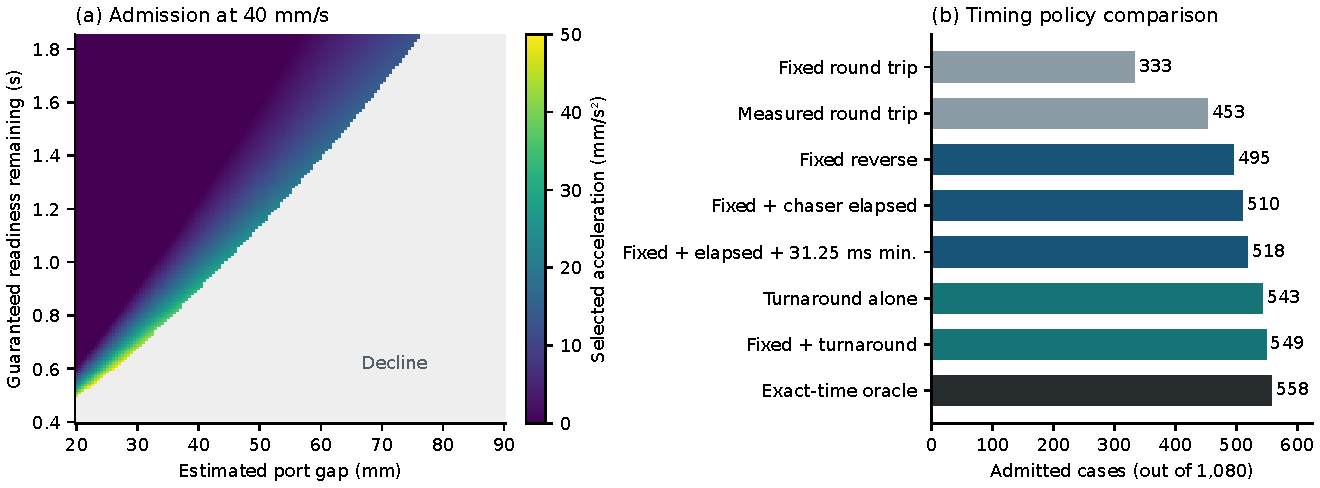
\includegraphics[width=\textwidth]{admission.pdf}
\caption{Certified first-contact admission region and timing policy comparison. (a) Minimum certified command at 40 mm/s. Gray indicates refusal. (b) Admissions on the same 1,080-point grid using the same robust certificate. The exact-time oracle supplies physical expiry while retaining all motion and uncertainty constraints.}
\label{fig:admission}
\end{figure*}

\subsection{Finite Port Radius at Fixed Tilt}

For an antipodal contact ring of radius $r_p$ tilted by at most $\theta_{\max}$, the leading point can be ahead of the ring center by up to $r_p\sin\theta_{\max}$. If the relative port orientation is fixed and the projected points remain over the receiving disk, the effective clearance to first contact is in
\begin{equation}
\left[g_- - r_p\sin\theta_{\max},\; g_+\right].
\label{eq:tilt}
\end{equation}
Use this interval for the stopping and contact bounds. The fixed offset shifts first-contact time without changing the point's axial speed. For the test geometry, a separate lateral margin keeps the projected ring over the disk. Rotation during the approach would also change a point's axial velocity. It requires a moving contact-surface model and a corresponding velocity bound.

\section{Evaluation}

\subsection{Timing Policy Grid}

The 1,080 deterministic decision points cross six gaps (24--90 mm), four closing speeds (28--46 mm/s), five readiness durations (0.9--2.1 s), and nine combinations of forward and reverse timing. The three times before grant creation are 62.5, 187.5 and 312.5 ms, each including 31.25 ms of outbound delay. The three times after creation are 31.25, 156.25 and 281.25 ms. The clock-rate allowance is 1,000 ppm per clock. All variants use the same state bounds and guidance certificate. The gap and speed errors are bounded by 0.6 mm and 1.2 mm/s, actuation lag by 31.25--62.5 ms, and relative acceleration disturbance by 8 mm/s$^2$. The contact-speed band is 20--70 mm/s, the inward command limit is 50 mm/s$^2$, and the handoff reserve is 40 ms.

Fig.~\ref{fig:admission} compares eight ways to supply the remaining-time bound to the same certificate. A fixed whole-exchange bound admitted 333 points and the measured whole exchange admitted 453. The stronger fixed reverse-delay bound admitted 495 points. Correcting the measured exchange for receiver turnaround admitted 543 points. Combining that estimate with the fixed reverse-delay bound admitted 549, compared with 558 for an oracle supplying exact physical expiry. The corrected estimate alone gained 54 grid points and lost six relative to fixed reverse delay (net 48). Combining the fixed bound with measured chaser elapsed time alone admitted 510 points. Using the grid's 31.25 ms processing minimum raised this to 518. Using measured turnaround with the fixed bound admitted 549. These counts characterize the constructed grid. Independently stepping 21,720 prescribed piecewise scalar trajectories found no violation of their certified time or speed intervals beyond floating-point roundoff. A separate 20,000-case clock and delay check found no violation of \eqref{eq:remaining}.

\subsection{OEL Software-in-the-Loop Testbed}
\label{sec:oel-testbed}

OEL propagated the translation and attitude of two synthetic 100 kg spacecraft with Earth two-body orbital dynamics. A generic ring-and-disk model coupled their motion at contact. The probe and receiving disk had radii of 0.20 and 0.25 m, respectively. The same simulation scheduler advanced separate chaser and receiver flight-software tasks every 31.25 and 62.5 ms, respectively. Study plug-ins implemented the readiness protocol and emulated each vehicle's local clock. The chaser received port measurements with assigned biases, and cases included axial acceleration of the receiver. The initial campaign and holdout used scripted message delivery. The comparator used a causal queue with configurable reply delays and losses.

The runs produced docking-event records and timestamped flight-software diagnostics. A separate scorer combined simulated first contact, soft capture and separation with the flight software's decision and reservation records. This let the scorer check expiry and capture margins using simulator time while the chaser based its decisions on local elapsed time and message contents. The 40 ms handoff is a modeled period after contact over which the receiver remains committed. The adaptive scorer checks for release or rebound during that period. The 40 ms value is an experimental allowance. Its flight value would be set by measured mechanism and controller timing. Supplement Sec.~S2 identifies the experimental OEL build and gives a reference replay.

\subsection{Initial Paired Runs and Negative Controls}

The 15 initial runs used emulated clock epochs separated by 1,291 s. The seven captures admitted under the complete certificate fell within their certified time and speed intervals and left at least 40 ms of readiness beyond the latest possible contact. Five refused approaches retained positive separation. The cases include two step sizes for the outward-moving receiver, which agreed on first-contact time. The three remaining runs isolate failures from removing an assumption or part of the certificate:
\begin{itemize}
\item Treating a delayed grant as fresh at receipt produced unarmed contact 248 ms after its physical expiry.
\item Breaking a valid readiness promise led to unarmed contact at the nominal time.
\item At 0.04 rad of fixed tilt, first contact occurred with nearly 8 mm of port-center clearance. It preceded the center-only earliest bound by 62 ms. Including \eqref{eq:tilt} enclosed the event.
\end{itemize}

\subsection{Prospective Boundary Holdout and Live Timing}

\begin{figure*}[!t]
\centering
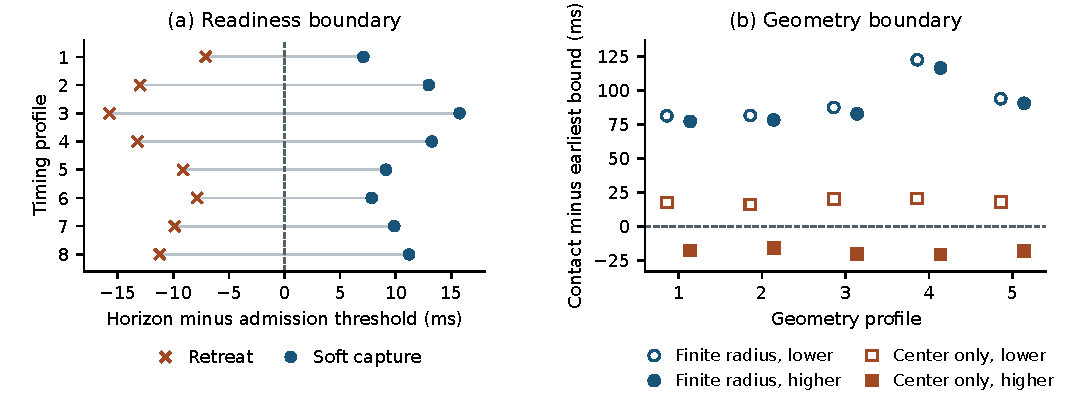
\includegraphics[width=\textwidth]{boundary-holdout.pdf}
\caption{Prospective holdout of the readiness and contact-geometry predictions in 36 OEL runs. (a) Each line joins two versions of one timing profile. The horizontal coordinate is the certified horizon relative to its predicted admission threshold. (b) Measured first-contact time minus the frozen earliest-contact prediction. Negative values indicate contact before the predicted window. All contacts occurred before their respective latest-contact bounds.}
\label{fig:holdout}
\end{figure*}

The frozen holdout plan recorded the source hashes, inputs, predicted outcomes and scoring tolerances. In Fig.~\ref{fig:holdout}(a), eight paired profiles changed only receiver promise duration, placing the encounters 7.1--15.7 ms on either side of the modeled admission boundary. All eight inside cases captured and all eight outside cases retreated, with at least 29.11 mm of sampled retreat clearance. For Fig.~\ref{fig:holdout}(b), the scalar forecast selected two tilts per geometry on opposite sides of the predicted center-only timing boundary before running OEL. OEL reproduced all five predicted higher-tilt crossings. Contact preceded the center-only earliest time by 16.1--20.7 ms. The five lower-tilt contacts stayed within the center-only bounds. The finite-radius bounds enclosed all ten contacts in the corrected runs.

Two processes exchanged messages through a local pipe, with clock rates and epochs emulated from one host monotonic clock. Four initial exchanges exercised valid, out-of-order, late and omitted replies. Twelve further exchanges bracketed the nominal threshold. The timestamp-based classifier agreed with all 12 decisions. Scheduling moved four of six nominally admissible trials across the boundary. The fixture inserts a 20 ms wait between the chaser's request timestamp and transmission. Across the two accepted trials here and six in the repeat, the expiry margin beyond latest contact and handoff matched the outbound interval from that timestamp to receiver receipt within 3 ns. The minimum margins of 22.613 and 22.584 ms reflect this fixture. The decision timestamp precedes certificate computation, so the recorded interval ends before computation and command delivery.

\subsection{Adaptive Fixed-Window Comparison}

The adaptive policies share a causal message queue, a 32 mm/s slowdown target while waiting, one renewal of up to 1.9 s, a 2 mm retreat reserve and a 40 ms handoff reserve. The receiver honors issued grants even if a reply is lost. All adaptive policies can use the 281.25 ms upper bound on grant-to-reply delay and age the grant on the chaser clock after receipt. We compare that fixed bound alone, its combination with chaser elapsed time assuming $P_{\min}=0$, and its combination with measured receiver turnaround. A fourth adaptive comparator uses elapsed time and the fixture-wide physical minimum $P_{\min}=62.5$ ms. It reads no receiver timing field. At each decision a policy uses the larger of its available lower bounds. A one-shot fixed policy and a renewable fixed policy that coasts while waiting provide additional comparisons.

Each policy runs 21 profiles. Eighteen cross three approach geometries, three delay settings, and two renewal caps. Three add lost first and renewal replies and an extended receiver turnaround. The score independently reconstructs grant expiry from receipt records, receiver issue telemetry and the assigned receiver clock rate. A successful run requires both ports armed at first contact, soft capture within the computed time and speed bounds, and a latest certified contact time at least 40 ms before expiry. A retreat requires no contact, the specified sampled clearance, and final opening motion.

\begin{table}[!t]
\caption{Matched adaptive comparison on 21 profiles per policy}
\label{tab:adaptive}
\centering
\small
\setlength{\tabcolsep}{3.8pt}
\begin{tabular}{@{}lrrrr@{}}
\toprule
Policy & Captures & First grant & Renewals & Retreats\\
\midrule
Fixed, one shot   & 10 & 10 &  0 & 11\\
Fixed, slow/renew & 15 & 10 & 11 &  6\\
Fixed, coast/renew& 15 & 10 & 11 &  6\\
Fixed + elapsed, adaptive & 17 & 15 & 6 & 4\\
Elapsed + 62.5 ms minimum & 20 & 20 & 1 & 1\\
Measured turnaround & 20 & 20 & 1 & 1\\
\bottomrule
\end{tabular}
\end{table}

Table~\ref{tab:adaptive} shows which timing assumptions changed the decision. Relative to fixed delay alone, elapsed time with $P_{\min}=0$ added the moving and tilted fast-link profiles with capped renewals. Measuring turnaround also admitted two level profiles with capped renewals and a profile with a lost renewal reply. Supplying the 62.5 ms minimum recovered the same three captures. Both policies completed the same 20 profiles on first grants, requested one renewal and occupied 25.65 s of receiver time in aggregate. Supplement Table S1 gives the original profile breakdown and Table S4 compares all four adaptive timing policies. In the original 84 runs, all 60 captures met their scoring criteria and all 24 retreats retained at least 4.160 mm of sampled leading-edge clearance (2 mm required). Two representative matched pairs reproduced the decisions, selected grants and contact times at half the physics and output steps.

For the 15 profiles completed by the corrected and renewable fixed-delay policies, the corrected method arrived 101--169 ms sooner than the faster successful fixed recovery strategy in five profiles where it avoided renewal, tied in six, and arrived 48--92 ms later in four. In the four slower profiles both methods used the first grant. The larger certified window allowed the shared objective to select less acceleration. In one moving receiver case the window increased from 0.898 to 0.991 s, the selected acceleration fell from 22.53 to 9.89 mm/s$^2$, and contact occurred 92 ms later.

\subsection{Reservation Sensitivity and Broader Sample}

To test whether the advantage depends on the grant schedule, we crossed three approach geometries with two initial durations (1.10 and 1.40 s), two renewal caps (0.85 and 1.90 s), and two renewal reply delays (52 and 201 ms). The first configured reply delay was 41 ms. The delays fall between scheduled task ticks, and decisions use actual delivery on the simulator scheduler. All timing policies faced the same grant limits for each profile. A short renewal cap represents limited reserve capacity for a new commitment after an initial interval has already been approved. The caps are experimental inputs for sensitivity analysis.

Across the 24 profiles, fixed delay alone yielded 18 captures and elapsed time with a zero processing minimum yielded 20. The known minimum and measured turnaround each yielded the same 22 captures, four renewals and 32.00 s of occupancy. With both grants short, fixed delay alone admitted zero profiles. Elapsed time with a zero minimum admitted both level profiles. The known minimum and measured turnaround each admitted the two level and two moving profiles. All four policies occupied 6.60 s in this group. With the larger renewal cap both completed all six short-initial-grant profiles. The corrected policy occupied 8.58 s across that group versus 12.53 s for the fixed policy. Both captured all 12 long-initial-grant profiles on their first grants. Occupied time is the union of issued reservations, including grants whose replies were lost, summed over runs. It quantifies the time for which the receiver is committed in this model. A scheduler bounding resources across multiple encounters would require additional analysis.

All four adaptive timing policies captured the same ten of 12 seeded profiles drawn without screening on the certificate's predictions. Measured turnaround used three renewals and occupied 18.04 s. The known-minimum policy used four and occupied 18.65 s. This sample also varies gap, speed, bias, lag, tilt, target acceleration and reply timing. It illustrates that the completion gain is sensitive to the profile design. Across the two batches and six refinements, all 64 captures and 14 retreats met the simulated scoring checks. Supplement Secs.~S3--S4 report the strata, paired comparisons and scoring details.

\subsection{Independent Checks on the Modeled Envelope}

For the 64 captures, we independently solved the axial contact equation using the simulator state at commitment, the commanded acceleration and the known receiver acceleration. The largest difference from OEL event time was 22.1~$\mu$s. Halving and quartering the integration and contact steps of three selected scenarios preserved their decisions and selected grants. For the two captures, the recorded event times agreed at all three settings. The third case was a retreat. The scheduler periods remained fixed. A further ten runs tested delayed approach and brake commands at five settings, including 46.875 ms between task ticks. Commands took effect on the first eligible chaser tick. The OEL applied-acceleration history gave 31.25 or 62.5 ms from decision to actuation, within the certified interval in all ten runs. The five approaches captured and all five braking cases retained the required leading-edge clearance.

At sampled approach times, the smallest disk overlap allowance $r_{\rm disk}-r_p-\lVert \mathbf{p}_{\rm lateral}\rVert$ was 44.0 mm. After removing the integral of the delayed chaser command, the largest sampled interval-averaged axial acceleration magnitude was 7.00 mm/s$^2$, below the 8 mm/s$^2$ bound. The relative angular rates recorded before contact were zero, and nonzero inward commands appeared at the configured onset in the flight-software diagnostics. The ideal wrench interface maps force to acceleration at the specified mass. These checks quantify agreement in the sampled simulated approaches. They provide no continuous-time bound for arbitrary attitude or actuator motion.

Independent numerical integration with 296 bounded sinusoidal disturbance histories found no violation of the contact envelopes on admitted scalar cases. On the original decision grid, 153 of 522 refusals by the exact-expiry robust certificate had a feasible nominal constant command under exact state and zero disturbance. This is a lower bound on the number of refusals that can succeed in that nominal comparison. It shows the conservatism of the robust constraints even when expiry is known. A repeat of the one-host IPC trial agreed with the timestamp-based classifier in all 12 exchanges and produced six admissions, compared with two in the earlier run.

\section{Discussion}

The interface specification determines the value of reporting turnaround. Section~\ref{sec:example} identifies two physically different deadlines that elapsed time alone cannot distinguish. Across the 57 closed-loop profiles, a guaranteed 62.5 ms processing minimum supplied enough information to match every capture and retreat decision of the measured-turnaround policy. First-contact times still differed in 31 profiles, and measured turnaround saved one renewal in the separately sampled cohort. A system using a fixed processing minimum must establish that grant issuance can never occur sooner, including under faster execution or revised scheduling.

In the original comparison and implementation-check batches, soft capture coincided with first contact in all 124 and 147 captures, respectively. The geometry test therefore bears directly on the timing of contact. Independent latch completion remains an experimental question.

The spatial envelope with moving ports and coupled actuation remains open. A bench investigation should measure actuator and link timing, log actual readiness expiry and contact on an independent reference clock, and freeze cases on both sides of the predicted boundaries. Prior hardware-in-the-loop docking studies also identify delay in the test apparatus as a source of contact-model error \cite{zebenay}. Fault-injection trials would test whether an actual receiver can retain arming and its motion envelope under reset or abort requests.

\section{Conclusion}

An expiring receiver commitment, a bound on grant age and a reachable first-contact window together give a decision rule for cooperative docking. The equal-observation example establishes when reporting turnaround makes a safe commitment possible. The closed-loop runs show when a simpler interface gives the same completion outcomes. A prospective tilt test shows why either timing policy must use the clearance of the first point that can touch the receiver.

\section*{Data and Code Availability}

The supplement gives per-profile outcomes, identifies the OEL build, and documents the reference replay and the revision studies. The accompanying evidence package contains machine-readable case data, analysis scripts, and compact event, clearance and actuation records for independent rescoring. It also includes the 57 known-minimum policy scores and code to reproduce the equal-observation example. Rerunning OEL trajectories requires access to the identified experimental checkout and compatible runtime. The local archive retains the review stores and configurations. The paper, supplement and study materials are available in the \href{https://github.com/adamcohen8/OEL-studies/tree/main/original-research/cooperative-docking}{OEL studies repository}.

\section*{Acknowledgment}

OpenAI Codex with GPT-6 assisted with the literature search, study design, derivations and checks in Sections~II--III, generation of study scripts and figures, analysis in Section~IV and the supplement, and drafting throughout. OEL and local deterministic verification scripts produced the simulation and analytical results. The author is responsible for checking the claims, sources, code, and wording.

\newpage
\bibliographystyle{IEEEtaes}
\bibliography{references}

\end{document}
